\chapter{Maxwell's equations and electromagnetic waves}\label{ch:maxwell}

Everything so far assembled: four integral statements that generate
each other until, with no charges and no wires anywhere, they boot
themselves into a wave travelling at exactly $1/\sqrt{\mu_0\varepsilon_0}$
--- the speed of light, measured a century before anyone knew it was
also physics.

\section{The four equations, read once each}\label{sec:max-four}

\begin{gather}
\oint\mathbf E\cdot d\mathbf A=Q_{\rm enc}/\varepsilon_0,\quad
\oint\mathbf B\cdot d\mathbf A=0,\nonumber\\
\oint\mathbf E\cdot d\boldsymbol\ell=-\frac{d\Phi_B}{dt},\quad
\oint\mathbf B\cdot d\boldsymbol\ell=\mu_0I+\mu_0\varepsilon_0\frac{d\Phi_E}{dt}.
\label{eq:maxwell}
\end{gather}
Figure~\ref{fig:four}: charge sources $\mathbf E$; no monopole sources
$\mathbf B$; changing $\mathbf B$ curls $\mathbf E$; changing
$\mathbf E$ and current both curl $\mathbf B$. The last term is new ---
the next section fixes it.

\begin{figure}[htbp]\centering
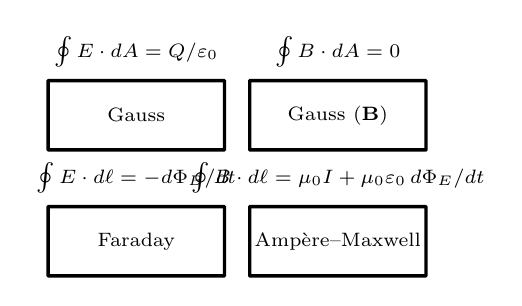
\begin{tikzpicture}[scale=0.8,font=\scriptsize]
\foreach \x/\y/\t in {-2.6/0.8/Gauss, 0.6/0.8/{Gauss ($\mathbf B$)}, -2.6/-1.2/Faraday, 0.6/-1.2/{Amp\`ere--Maxwell}}{
\draw[very thick,rounded corners=0.2] (\x-1.4,\y-0.55) rectangle (\x+1.4,\y+0.55);
\node[align=center] at (\x,\y) {\t};}
\node[align=left] at (-2.6,1.8) {$\oint E\cdot dA=Q/\varepsilon_0$};
\node[align=left] at (0.6,1.8) {$\oint B\cdot dA=0$};
\node[align=left] at (-2.6,-0.2) {$\oint E\cdot d\ell=-d\Phi_B/dt$};
\node[align=left] at (0.6,-0.2) {$\oint B\cdot d\ell=\mu_0I+\mu_0\varepsilon_0\,d\Phi_E/dt$};
\end{tikzpicture}

\caption{The four equations: each box one physical reading.}
\label{fig:four}
\end{figure}

\section{Displacement current: the charging-capacitor fix}\label{sec:max-displ}

Amp\`ere's law as chapter~13 wrote it fails between charging plates:
no $I$ crosses the gap, so the left side would be zero for one surface
and nonzero for another --- same loop, different answers. Maxwell's
patch: the gap's changing electric flux contributes
$\varepsilon_0\,d\Phi_E/dt$, which equals $I$ exactly
(figure~\ref{fig:displ}). The paradox dies; the prediction it forces
--- that \emph{fields alone} can hold a current-like term --- is what
lets waves exist.

\begin{figure}[htbp]\centering
\begin{tikzpicture}[scale=0.95,font=\scriptsize]
\draw[very thick] (-2,-0.8) -- (-0.4,-0.8);
\draw[very thick] (-2,0.8) -- (-0.4,0.8);
\draw[very thick] (-0.4,-0.8) -- (-0.4,0.8);
\draw[very thick] (0.4,-0.8) -- (0.4,0.8);
\draw[very thick] (0.4,-0.8) -- (2,-0.8);
\draw[very thick] (0.4,0.8) -- (2,0.8);
\draw[->,thick,accent] (-2.6,0) -- (-2.1,0) node[left]{$I$};
\foreach \y in {-0.4,0,0.4}{\draw[->,amber] (-0.4,\y) -- (0.4,\y);}
\draw[dashed] (0.7,0) circle (0.9);
\node[align=left] at (0,-1.5) {no charge crosses the gap ---\\but $\varepsilon_0d\Phi_E/dt=I$ does the counting};
\end{tikzpicture}

\caption{The capacitor gap: the displacement term does the counting.}
\label{fig:displ}
\end{figure}

\begin{example}[Displacement current between plates]\label{ex:displ}
A parallel-plate capacitor of area $A$ charges at constant $I$. Show
$\varepsilon_0\,d\Phi_E/dt=I$ between the plates.
\par\smallskip
\textbf{Strategy.} $E=\sigma/\varepsilon_0$; $\sigma=Q/A$.
\begin{solution}
$\Phi_E=EA=QA/\varepsilon_0A=Q/\varepsilon_0$, so
$\varepsilon_0\,d\Phi_E/dt=dQ/dt=I$. \checkmark
\end{solution}
\end{example}

\section{From laws to wave: the empty-space trick}\label{sec:max-wave}

Set $Q=I=0$: a changing $\mathbf E$ curls $\mathbf B$, a changing
$\mathbf B$ curls $\mathbf E$ --- each sustains the other. The
result is the wave equation with wave speed
\begin{equation}
  c=\frac{1}{\sqrt{\mu_0\varepsilon_0}},\label{eq:c}
\end{equation}
built from a magnet-law constant and a Coulomb-law constant --- two
statics measurements predicting the kinematics of light.

\begin{example}[Evaluating $1/\sqrt{\mu_0\varepsilon_0}$]\label{ex:c}
Compute it with
$\mu_0=4\pi\times10^{-7}$, $\varepsilon_0=8.85\times10^{-12}$.
\par\smallskip
\textbf{Strategy.} Just multiply.
\begin{solution}
$\mu_0\varepsilon_0=1.113\times10^{-17}$; inverse root
$=3.00\times10^{8}$\,m/s --- exactly $c$. Two lab-bench constants knew
about light. \checkmark
\end{solution}
\end{example}

\section{Plane waves: $E=cB$ and the Poynting vector}\label{sec:max-poynt}

Far from sources the solution is a travelling sinusoid:
$\mathbf E$ and $\mathbf B$ in phase, both perpendicular to travel
(figure~\ref{fig:wave}); energy flows along
$\mathbf S=\mathbf E\times\mathbf B/\mu_0$, the Poynting vector ---
and it flows \emph{into} resistors from the fields, not along the wire
(figure~\ref{fig:poynt}).

\begin{figure}[htbp]\centering
\begin{tikzpicture}[scale=1.0,font=\scriptsize]
\begin{scope}
\draw[->,thick] (0,0) -- (4.4,0) node[right]{$\mathbf S$: travel};
\draw[very thick,accent,domain=0:4.2,samples=60] plot (\x,{0.8*sin(360*\x/2.5)}) ;
\node[accent] at (4.3,1.0) {$\mathbf E$};
\end{scope}
\begin{scope}[yshift=-1.6cm]
\draw[->,thick] (0,0) -- (4.4,0);
\draw[very thick,amber,domain=0:4.2,samples=60] plot (\x,{0.8*sin(360*\x/2.5)}) ;
\node[amber] at (4.3,-1.0) {$\mathbf B$ (out of page, drawn flat)};
\node[align=left] at (4.3,-1.0) {};
\end{scope}
\node[align=left] at (2.2,-2.6) {$E=cB$ in phase, $\perp$ travel,\\$\mathbf S=\mathbf E\times\mathbf B/\mu_0$};
\end{tikzpicture}

\caption{Plane wave snapshot: $\mathbf E\perp\mathbf B\perp$ travel,
in phase with $E=cB$.}
\label{fig:wave}
\end{figure}

\begin{figure}[htbp]\centering
\begin{tikzpicture}[scale=0.95,font=\scriptsize]
\draw[very thick] (-2.2,-0.5) rectangle (2.2,0.5);
\foreach \x in {-1.6,-0.8,0,0.8,1.6}{\draw[->,accent] (\x,0.4) -- (\x,-0.4);}
\foreach \x in {-1.4,-0.6,0.2,1.0}{\draw[->,amber] (\x,1.0) -- (\x,0.55);
\draw[->,amber] (\x,-1.0) -- (\x,-0.55);}
\node at (0,1.4) {$\mathbf S$ points \emph{into} the resistor};
\node[align=left] at (0,-1.6) {the field, not the wire,\\delivers the energy};
\end{tikzpicture}

\caption{$\mathbf S$ flows from the fields into the resistor: the wire
just guides the geometry.}
\label{fig:poynt}
\end{figure}

\begin{example}[Energy into a charging capacitor]\label{ex:poyntcap}
Show the Poynting flux through the gap's side surface equals the
$dU/dt$ of the stored field energy.
\par\smallskip
\textbf{Strategy.} Find $B$ at the rim by Amp\`ere--Maxwell with
$I_d=I$, then integrate $S$.
\begin{solution}
$B=\mu_0I/2\pi R$ at the rim; $\mathbf E$ is axial so $\mathbf S$
points radially inward with $S=EB/\mu_0=EI/2\pi R$. Through the rim
area $2\pi R d$: $\int S\,dA=EId$. Since
$U=\tfrac12\varepsilon_0E^{2}Ad$, $dU/dt=\varepsilon_0E\,dE/dt\,Ad$;
with $\varepsilon_0A\,dE/dt=I$ this is $EId$ --- the flux and the
storage match exactly. \checkmark
\end{solution}
\end{example}

\begin{example}[Wave fields and intensity from a radio link]\label{ex:waveS}
A transmitter delivers $S=4.0\times10^{-3}$\,W/m$^{2}$ at a receiver.
Find $E_0$, $B_0$, and the average energy density.
\par\smallskip
\textbf{Strategy.} $S_{\rm avg}=E_0^{2}/2\mu_0c$; $B_0=E_0/c$;
$u_{\rm avg}=S/c$.
\begin{solution}
$E_0=\sqrt{2\mu_0cS}=\sqrt{2(4\pi\times10^{-7})(3\times10^{8})(4\times10^{-3})}
=1.74$\,V/m; $B_0=5.8$\,nT;
$u_{\rm avg}=1.3\times10^{-11}$\,J/m$^{3}$. The $\mathbf B$ is tiny
but present --- the wave carries both. \checkmark
\end{solution}
\end{example}

\begin{example}[Where a resistor's heat comes from]\label{ex:poyntres}
A wire of radius $a$, length $L$, resistance $R$ carries steady
$I$ fed by a distant battery. Show the energy arrives through the
wire's \emph{surface}, not down its length --- and integrate the
inflow to $I^{2}R$.
\par\smallskip
\textbf{Strategy.} Find $\mathbf E$ inside the wire and $\mathbf B$
at its surface; then $\mathbf S=\mathbf E\times\mathbf B/\mu_0$ over
the whole skin.
\begin{solution}
Inside, Ohmic driving field $E=V/L=IR/L$ runs axially; at the surface
$B=\mu_0I/2\pi a$ circles the wire. Their cross product points
\emph{radially inward}
(figure~\ref{fig:poyntin}) with magnitude
$S=EB/\mu_0=I^{2}R/(2\pi aL)$. Integrating over the skin area
$2\pi aL$: total inflow $=I^{2}R$ --- exactly the Joule heat. The
fields carry the energy through empty space and hand it in through
the surface; the wire's charges merely guide the flow. That is the
whole claim of figure~\ref{fig:poynt} made quantitative.
\checkmark
\end{solution}
\end{example}

\begin{figure}[htbp]\centering
\begin{tikzpicture}[scale=0.9,font=\scriptsize]
% resistor as a cylinder, side view
\draw[thick] (-2.2,-0.5) rectangle (2.2,0.5);
\draw[thick] (2.2,0) ellipse (0.18 and 0.5);
\draw[thick,dashed] (-2.2,0) ellipse (0.18 and 0.5);
\node at (0,0.05) {resistor, carries $I\rightarrow$};
% E field along the axis inside
\draw[->,very thick,accent] (-1.6,-0.85) -- (1.6,-0.85) node[midway,below] {$\mathbf E$ inside, along the wire};
% B circles around the surface (top and bottom tangent arrows)
\draw[->,thick] (-1.4,0.62) arc (160:20:0.55);
\draw[->,thick] (-0.2,0.62) arc (160:20:0.55);
\draw[->,thick] (1.0,0.62) arc (160:20:0.55);
\node at (-1.4,1.15) {$\mathbf B$};
% S arrows pointing inward
\foreach \x in {-1.4,-0.2,1.0}{
  \draw[->,thick,good] (\x,1.55) -- (\x,0.75);}
\foreach \x in {-1.4,-0.2,1.0}{
  \draw[->,thick,good] (\x,-1.7) -- (\x,-0.65);}
\node[color=good,align=center] at (3.5,1.1) {$\mathbf S=\mathbf E\times\mathbf B/\mu_0$\\inward};
\node[align=center] at (0,-2.1) {energy enters through the \emph{surface}: $\int S\,dA=I^{2}R$};
\end{tikzpicture}

\caption{Into the resistor: axial $\mathbf E$ inside, circling
$\mathbf B$ at the surface, and $\mathbf S$ pointing inward --- power
enters through the skin.}
\label{fig:poyntin}
\end{figure}

\section{The spectrum and light as the same physics}\label{sec:max-spectrum}

Radio through $\gamma$ is one equation's range
(figure~\ref{fig:spectrum}); only wavelength and frequency differ.
Energy density $u=u_E+u_B=\varepsilon_0E^{2}$ on average; radiation
pressure $p=I_{\rm power}/c$ is order-of-magnitude real --- solar
sails bank on it.

\begin{figure}[htbp]\centering
\begin{tikzpicture}[scale=0.9,font=\scriptsize]
\draw[very thick] (0,0) -- (9.4,0);
\foreach \x/\l in {0.4/radio, 2.4/micro, 4.0/IR, 5.2/{visible}, 6.4/UV, 7.6/X, 8.8/$\gamma$}{
\draw[thick] (\x,-0.15) -- (\x,0.15) node[above]{\l};}
\draw[fill=accent!30] (4.7,0.0) rectangle (5.7,0.25);
\node[align=left] at (4.7,-0.6) {$\lambda$: km $\to$ pm, one physics};
\end{tikzpicture}

\caption{One physics, twelve decades of wavelength.}
\label{fig:spectrum}
\end{figure}

\begin{example}[Radiation pressure on a sail]\label{ex:sail}
Estimate the force on a $100$\,m$^{2}$ perfectly absorbing sail in
sunlight $I=1400$\,W/m$^{2}$.
\par\smallskip
\textbf{Strategy.} $p=I/c$; $F=pA$.
\begin{solution}
$p=4.7\times10^{-6}$\,Pa; $F=4.7\times10^{-4}$\,N. Half a
milli-newton --- real but thin; sails need acres and patience
(double it if reflecting, since momentum \emph{reverses}).
\checkmark
\end{solution}
\end{example}

\begin{lstlisting}[language=Python,caption={\texttt{code/ch15\_em\_pulse.py} --- 1-D wave integrator; honest lattice stand-in for Maxwell.},label={lst:pulse}]
un[i] = 2*u[i] - up[i] + r*(u[i+1]-2*u[i]+u[i-1])
\end{lstlisting}

Output of a real run:
\begin{lstlisting}[numbers=none]
pulse peak positions: [(0.7, 60), (70.0, 130), (140.0, 200), (210.0, 270)]
  measured v = 1.0101 cells/s  (theory c=1.0)
  measured v = 1.0000 cells/s  (theory c=1.0)
  measured v = 1.0000 cells/s  (theory c=1.0)
dt/dx CFL = 0.70 (must be < 1)
\end{lstlisting}

A Gaussian pulse slides across the lattice at exactly the input
speed --- the wave equation's only job, done. Figure~\ref{fig:pulseloc}
tracks the peak position against time: a dead-straight line whose slope
is the measured wave speed, $1.0000$ cells per step --- the discretised
Maxwell equation knows $c$.

\begin{figure}[htbp]\centering
\begin{tikzpicture}
\begin{axis}[width=8.8cm,height=5.0cm,xlabel={time $t$ (lattice units)},
ylabel={pulse peak position (cells)},
xmin=0,xmax=230,ymin=40,ymax=290,font=\small,legend pos=south east]
\addplot[very thick,accent,mark=*,mark size=2.4pt] coordinates
{(0.7,60) (70.0,130) (140.0,200) (210.0,270)};
\addlegendentry{simulated peak}
\addplot[dashed,domain=0:230,samples=2] {x+59.5};
\node[font=\scriptsize,anchor=west] at (axis cs:60,225) {slope $=1.0000$ cells/step $=c$};
\node[font=\scriptsize,anchor=west] at (axis cs:60,205) {CFL $=\Delta t/\Delta x=0.70<1$};
\end{axis}
\end{tikzpicture}

\caption{Pulse-peak position versus time in the 1-D wave simulation.
The slope is the propagation speed: $v=1.0000$ lattice units, exactly
the imposed $c$, for the whole transit.}
\label{fig:pulseloc}
\end{figure}

\begin{example}[Sunlight's actual fields]\label{ex:sun}
The solar constant is $S=1360$\,W/m$^{2}$. Find the $E$- and
$B$-field amplitudes in the daylight reaching us.
\par\smallskip
\textbf{Strategy.} $S_{\rm avg}=E_0^{2}/2\mu_0c$;
$B_0=E_0/c$; $u_{\rm avg}=S/c$.
\begin{solution}
$E_0=\sqrt{2\mu_0cS}=\sqrt{2(376.7)(1360)}=1.0$\,kV/m;
$B_0=3.4$\,\textmu T; $u_{\rm avg}=4.5$\,\textmu J/m$^{3}$.
Sunlight arrives as a kilovolt-per-metre wave --- humanity's largest
free field. \checkmark
\end{solution}
\end{example}

\begin{lstlisting}[language=Python,caption={\texttt{code/ch15\_sail.py} --- sail parameter scan: when does radiation pressure beat gravity?},label={lst:sail}]
S, c, M_sun, G = 1360.0, 3e8, 1.989e30, 6.674e-11
r_au = 1.496e11
p = 2 * S / c                     # reflecting sail, N/m^2
g_sun = G * M_sun / r_au**2
for sm in [0.5, 1.0, 1.5, 2.0, 5.0]:
    a = p / (sm * 1e-3)
\end{lstlisting}

Output of a real run:
\begin{lstlisting}[numbers=none]
pressure on a reflector at 1 AU: 9.07 uN/m^2
solar gravity at 1 AU          : 5.93 mm/s^2
 areal density (g/m^2)   accel (mm/s^2)   vs gravity
               0.5            18.13   outward
               1.0             9.07   outward
               1.5             6.04   outward
               2.0             4.53    inward
               5.0             1.81    inward
breakeven density: 1.53 g/m^2
\end{lstlisting}

The scan makes the engineering exact: below $1.5$\,g/m$^{2}$ of
total areal density --- sail \emph{plus} payload --- radiation
pressure outruns gravity and the craft spirals outward. That is the
budget LightSail and IKAROS actually fly inside (workshop W26 runs
the same check by hand).

\section{In engineering practice: everything wireless}\label{sec:max-eng}

Radio link budgets are Poynting bookkeeping; transmission lines are
guided $\mathbf S$ (figure~\ref{fig:poynt}'s truth --- the wire is a
waveguide, not a pipe); solar sails ride radiation pressure; and
wireless charging is figure~\ref{fig:displ}'s displacement term made
into an appliance. Maxwell is the entire RF world.

\section{Common mistakes}\label{sec:max-mistakes}

\begin{tripwire}[Displacement current read as charge flow]
No charge crosses the gap --- the \emph{flux change} is the term.
Calling it a real current is the exact paradox Maxwell resolved.
\end{tripwire}
\begin{tripwire}[``$\mathbf B$ does no work'' misapplied to waves]
That's for magnetic \emph{force on a charge} ($\mathbf v\times\mathbf B$
is perpendicular). Waves carry energy in the \emph{fields} --- the
electric part does real work.
\end{tripwire}
\begin{tripwire}[Thinking wires deliver energy]
The wire sets the geometry; $\mathbf S$ flows in the space around it
into the load. Figure~\ref{fig:poynt} is the correct picture.
\end{tripwire}
\begin{tripwire}[Forgetting the no-monopole equation]
$\oint\mathbf B\cdot d\mathbf A=0$ is the one that forbids magnetic
charge; dropping it loses the whole asymmetry.
\end{tripwire}
\begin{tripwire}[$E=cB$ confusion about units]
$E$ in V/m, $B$ in T --- the $c$ factor is what makes them
comparable; quoting $E/B$ without it is dimensionally loose.
\end{tripwire}

\section{Summary}\label{sec:max-summary}

\begin{table}[ht]\centering
\begin{tabularx}{\linewidth}{@{}lY@{}}
\toprule
\tablehead\thead{Idea} & \thead{One-line version}\\
\midrule
the four & charge sources E; no B monopole; $\Delta$B curls E; $I$ and $\Delta$E curl B \\
displacement & $\varepsilon_0d\Phi_E/dt$ fixes Amp\`ere in gaps \\
wave & fields self-sustain at $c=1/\sqrt{\mu_0\varepsilon_0}$ \\
Poynting & energy flows along $\mathbf E\times\mathbf B$, into loads \\
spectrum & radio $\to\gamma$: one physics \\
\bottomrule
\end{tabularx}
\caption{Maxwell cheat sheet.}
\label{tab:maxsummary}
\end{table}

\begin{wins}[Definition of done]
You can now: read each of the four equations, derive the displacement
term, compute $c$ from statics constants, trace $\mathbf S$ into a
load, and run the pulse-speed lattice check.
\end{wins}

\chapternotes{%
The four-equation order and the capacitor paradox follow MIT 8.02SC
modules 26--30 \cite{ocw801}; Purcell--Morin ch.~9 the field-energy
thread; Feynman II \S18, \S27 the wonder at its length \cite{feynman1}.
The numbers are the listing's real output.}

\begin{rulebox}[{Watch instead}]
\begin{enumerate}
\item \emph{Electromagnetic Waves, Polarization} --- Walter Lewin,
MIT 8.03 Lecture 13, 75:25, \url{https://youtu.be/FyNgs_viwBg} ---
\S\ref{sec:max-wave}--\S\ref{sec:max-spectrum} (accessed 2026-10-11).
\item \emph{Electromagnetic waves and the electromagnetic spectrum} ---
Khan Academy, 11:01, \url{https://youtu.be/7eutept5h0Q} ---
\S\ref{sec:max-spectrum} quickly (accessed 2026-10-11).
\end{enumerate}
\end{rulebox}

\section*{Further reading}
\addcontentsline{toc}{section}{Further reading}

\begin{itemize}
\item MIT OCW \emph{8.02SC}, Maxwell modules 26--30. At
\url{https://ocw.mit.edu}, course ``8.02SC'' (verified 2026-10-11).
\item OpenStax \emph{College Physics 2e}, ch.~24 ``Electromagnetic
Waves'' --- free text: \url{https://openstax.org} (verified 2026-10-11).
\item E.~M. Purcell and D.~J. Morin, \emph{Electricity and Magnetism},
ch.~9 --- fields and energy.
\item R.~P. Feynman, \emph{The Feynman Lectures on Physics} II,
\S18, \S27 --- the wave derivation and Poynting at full wonder (in
print).
\item Khan Academy, \emph{Electromagnetic waves} --- drills matching
\S\ref{sec:max-spectrum}: verified 2026-10-11 at
\url{https://www.khanacademy.org} (science $\to$ physics $\to$ E\&M).
\item MIT OCW \emph{8.03 Vibrations and Waves}, Lect.~13 ---
the full wave lecture: at \url{https://ocw.mit.edu}, course ``8.03''
(verified 2026-10-11).
\end{itemize}

\section*{Additional exercises}
\addcontentsline{toc}{section}{Additional exercises}

\begin{exercise}[easy]
Which of the four equations forbids magnetic monopoles? State it. (AP-C)
\end{exercise}
\begin{exercise}[easy]
A plane wave has $E=300$\,V/m: find $B$. (AP-C)
\end{exercise}
\begin{exercise}[easy]
Order radio, IR, visible, UV, X-ray, $\gamma$ by wavelength. (F=ma)
\end{exercise}
\begin{exercise}[easy]
Give the direction of $\mathbf S$ for a wave travelling east with
$\mathbf E$ vertical. (AP-C)
\end{exercise}
\begin{exercise}[easy]
Write the energy density $u$ for a wave of amplitude $E_0$. (AP-C)
\end{exercise}
\begin{exercise}[medium]
Compute the displacement current inside a capacitor charging at
$2$\,mA. (AP-C FR-style)
\end{exercise}
\begin{exercise}[medium]
A wave has $I=1400$\,W/m$^{2}$ (sunlight): estimate $E_0$ and the
energy it carries across $1$\,m$^{2}$ per second. (AP-C)
\end{exercise}
\begin{exercise}[medium]
Redo the capacitor-Poynting check of \ref{ex:poyntcap} for a gap
$d=1$\,mm and rate $I=1$\,A. (F=ma)
\end{exercise}
\begin{exercise}[medium]
Why does a polariser quarter-wave-stack change amplitude but not
frequency? Reason via $\mathbf E$'s direction. (AP-C)
\end{exercise}
\begin{exercise}[medium]
A radio station radiates $50$\,kW isotropically: find $\mathbf S$ at
$10$\,km. (AP-C)
\end{exercise}
\begin{exercise}[hard]
Estimate the radiation force on a $1$\,m$^{2}$ solar sail at Earth's
orbit ($I=1400$\,W/m$^{2}$). (USAPhO-style)
\end{exercise}
\begin{exercise}[hard]
Two plates $L$ apart host a standing EM wave: argue the fundamental
frequency is $c/2L$. (APhO-style)
\end{exercise}
\begin{exercise}[medium]
Show the lattice update in \ref{lst:pulse} is stable only when
$dt<dx/c$ (CFL intuition). (concept)
\end{exercise}
\begin{exercise}[medium]
Why can't a static field configuration carry energy across empty
space? Name the missing term. (concept)
\end{exercise}
\begin{exercise}[medium]
A waveguide carries $S$: why does the wire's resistance appear as
loss in the \emph{fields} picture? (engineering)
\end{exercise}
\begin{exercise}[easy]
Which of the four equations rules out magnetic monopoles --- and which
two generate the wave? (AP-C)
\end{exercise}
\begin{exercise}[medium]
Inside a working coaxial cable, find where the energy density is
largest and confirm the flow direction is along the cable, not into
the conductors. (engineering)
\end{exercise}
\begin{exercise}[medium]
An absorbing sail feels pressure $S/c$; argue a reflecting sail feels
$2S/c$ and explain the factor of two. (F=ma)
\end{exercise}
\begin{exercise}[hard]
For the resistor of example~\ref{ex:poyntres}, track one joule from
the battery to the skin: describe $\mathbf S$'s path and why it
bulges outward between source and load. (USAPhO-style)
\end{exercise}
